% Copyright 2023 The terCAD team. All rights reserved.
% Use of this content is governed by a CC BY-NC-ND 4.0 license that can be found in the LICENSE file.

\documentclass[12pt, a4paper, twoside]{extreport}
\setlength{\headheight}{17.0pt}
% Notes: Level of content
% -1 	\part{part}
% 0 	\chapter{chapter}
% 1 	\section{section}
% 2 	\subsection{subsection}
% 3 	\subsubsection{subsubsection}
% 4 	\paragraph{paragraph}
% 5 	\subparagraph{subparagraph}
\setcounter{tocdepth}{3}
\setcounter{secnumdepth}{3}
\usepackage[OT1]{fontenc}
\usepackage[utf8]{inputenc}
\usepackage[english]{babel}
\usepackage{amsmath}
\usepackage{amsfonts}
\usepackage{amssymb}
\usepackage{makeidx}
\usepackage{fancyhdr}
\usepackage{graphicx}
\graphicspath{ {./} }
\usepackage{watermark}
\usepackage{titling}
\usepackage[fencedCode,hashEnumerators,smartEllipses]{markdown}
\usepackage{lipsum}
\usepackage{tocloft}
\setlength{\cftsecindent}{0pt}
\setlength{\cftsubsecindent}{0pt}
\setlength{\cftsubsubsecindent}{0pt}
\cftsetindents{paragraph}{0em}{5em}
\usepackage{listings}
\usepackage{hyperref}
\usepackage{cleveref}
\crefname{figure}{Figure}{Figures}
\crefname{table}{Table}{Tables}
\crefname{listing}{Listing}{Listings}
\crefname{section}{Section}{Sections}
\usepackage{multicol}
\usepackage{pgfplots}
\usepackage{tabularx}
\usepackage{dirtree}
\renewcommand\DTstyle{\rmfamily}
\usepackage{wallpaper}
\usepackage[export]{adjustbox}

\usepackage{_lib/customization}
\usepackage{_lib/code-style}
%% Conversion to eBook
%\usepackage{ebook}

\sloppy

% Creating headers
\pagestyle{fancy}
\fancyhf{}
\fancyhead{}
\makeatletter
\renewcommand{\chaptermark}[2]{\markboth{\tiny #1}{\tiny #2}}
\makeatother

\fancyhead[LE]{\thepage}
\fancyhead[RE]{\itshape\nouppercase  \rightmark}
\fancyhead[LO]{\itshape\nouppercase \leftmark}
\fancyhead[RO]{\thepage}

\author{Viachaslau Lyskouski}
\title{From Zero to Market with Kotlin Multiplatform}
%\subtitle{Desktop, Mobile, and Web Distribution}
\date{2024}

% Reverse margins for the print version
\let\tmp\oddsidemargin
\let\oddsidemargin\evensidemargin
\let\evensidemargin\tmp
\reversemarginpar

\begin{document}
%% Conversion to eBook
%\ebook 

\maketitle
%\thispagestyle{empty}
%\ThisCenterWallPaper{1}{_cover/main.png}
%~
%\newpage

% Copyright 2023 The terCAD team. All rights reserved.
% Use of this content is governed by a CC BY-NC-ND 4.0 license that can be found in the LICENSE file.

\thispagestyle{empty}

\begin{figure}
  \begin{minipage}{0.49\textwidth}
    \large From Zero to Market with Kotlin Multiplatform\\
    \vspace{9mm}
    \noindent \small Desktop, Mobile, and Web Distribution\\
    \vspace{10mm}
    Viachaslau Lyskouski, 2024\\
    \vspace{2mm}
  \end{minipage}
  \hfill
  \begin{minipage}{0.41\textwidth}
    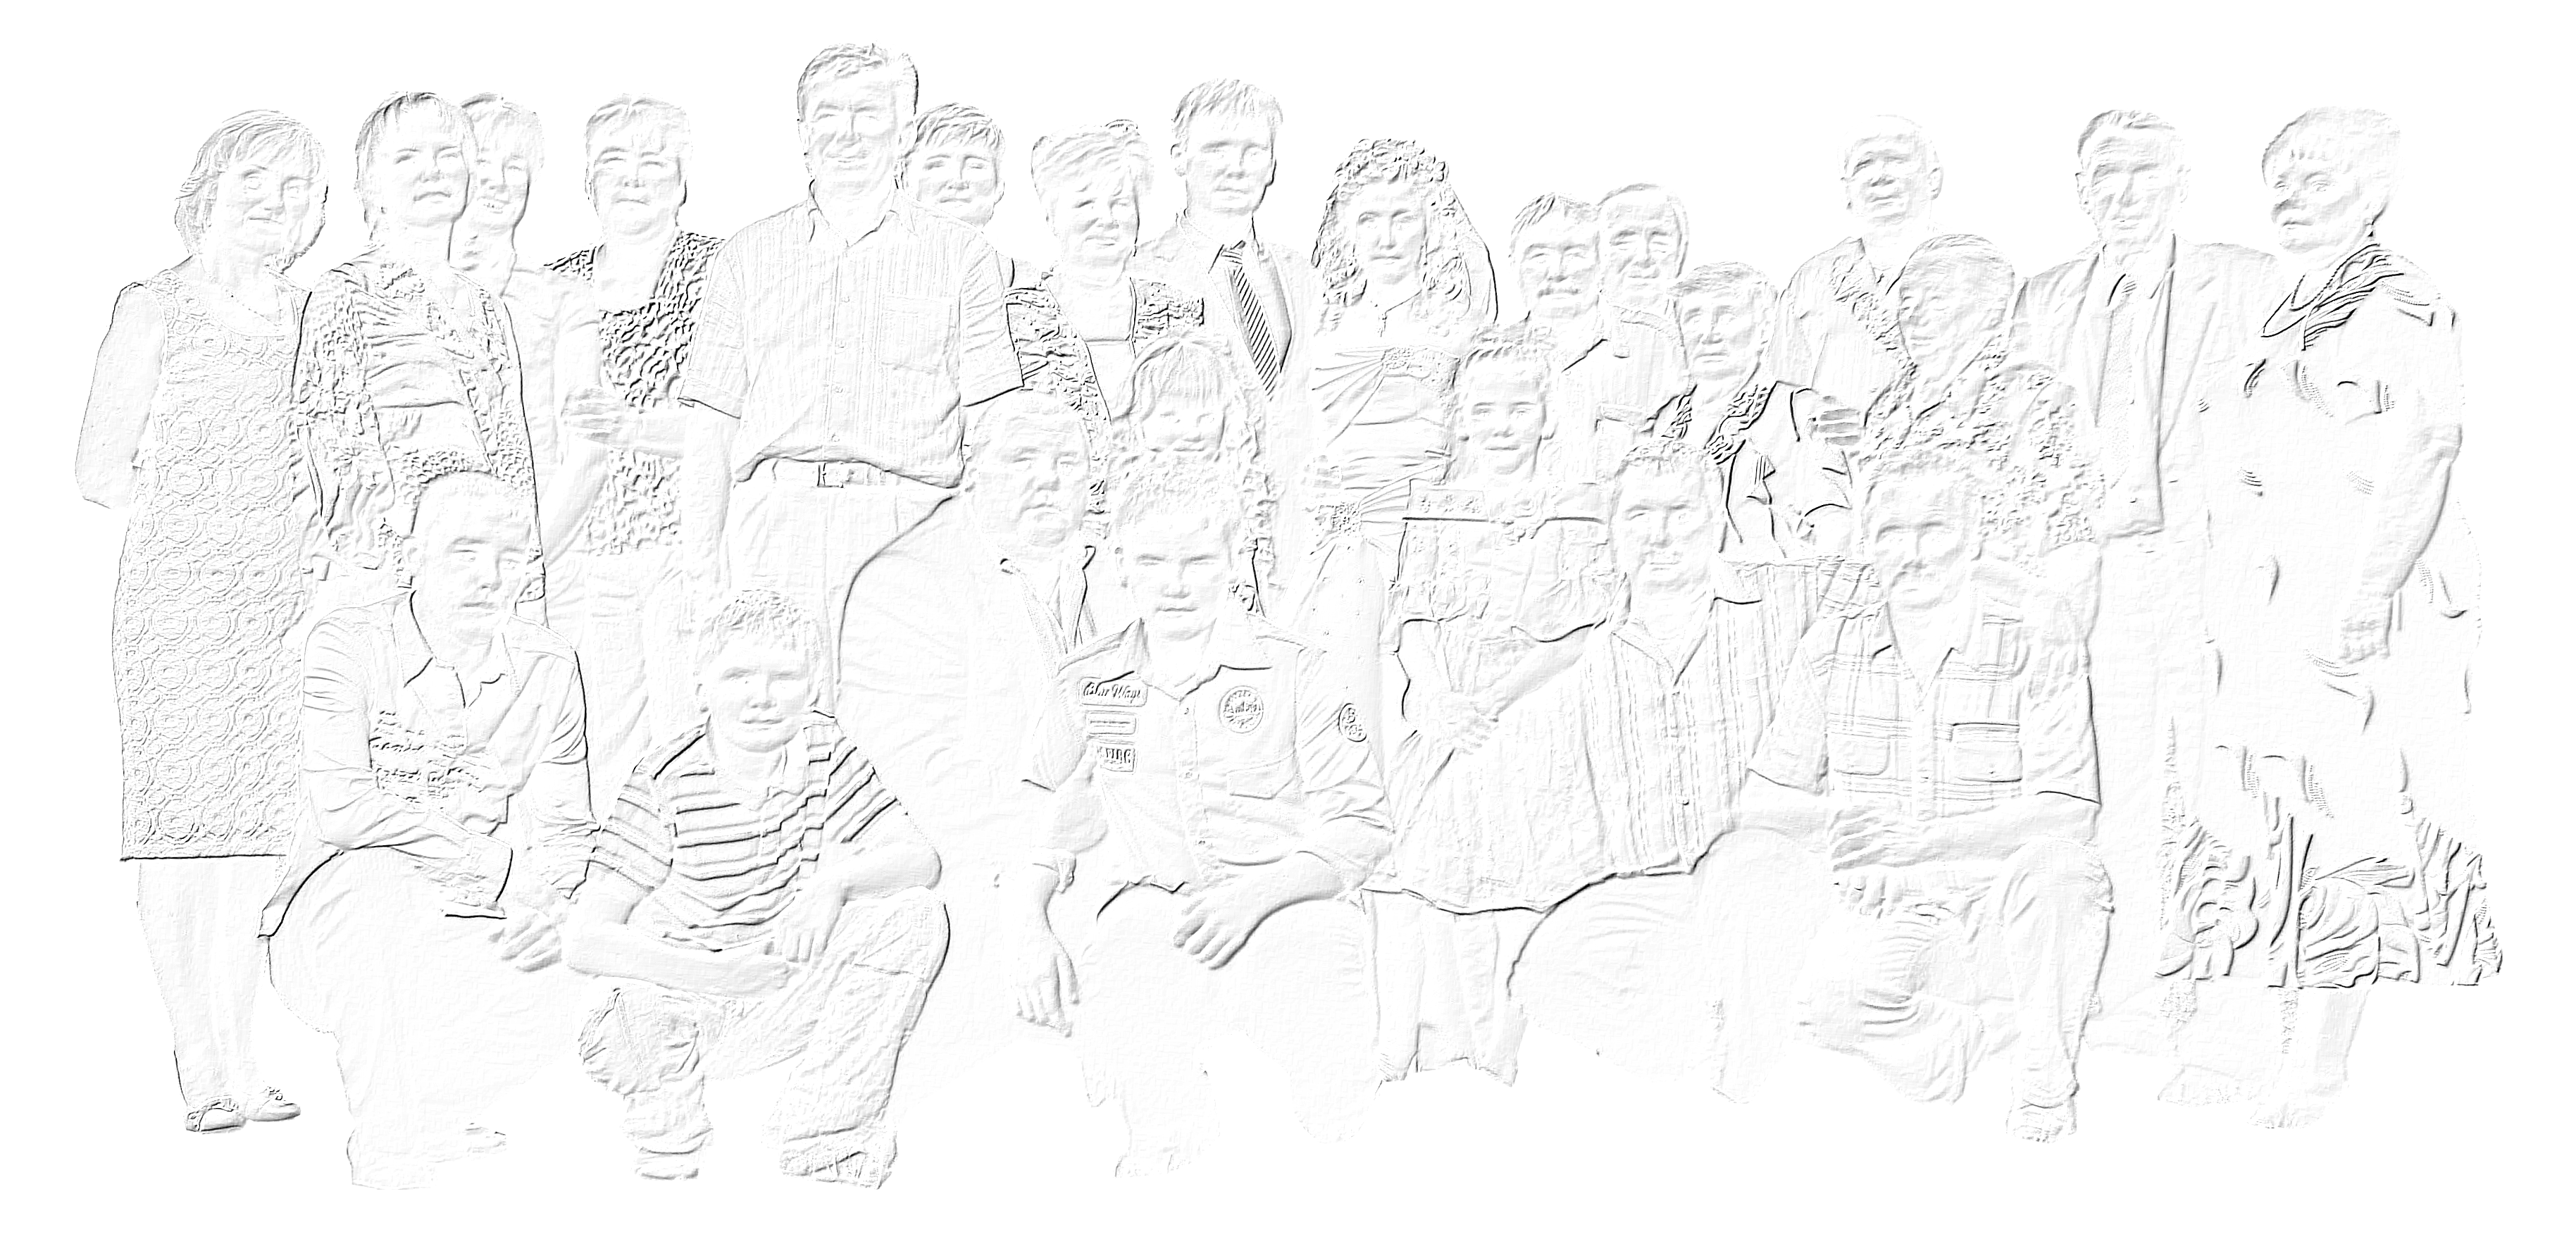
\includegraphics[width=\textwidth]{_cover/to.png}
    \emph{Dedicated to my Family}\\
  \end{minipage}
\end{figure}
~
\vspace{2cm}

\noindent The purpose of this book is not merely to instruct but to embark on a shared journey into the realm of 
platform-agnostic application development using Kotlin Multiplatform (KMP). I've started that book by knowing nothing 
about KMP and Kotlin, and the spent time have given me just an initial impulse to the mastery, but I still have 
something to share with you. 

\vspace{3mm}

\noindent I am confident that the time spent on coding (approximately 200 hours) can suffice for grasping the 
fundamental concepts of any programming language or framework, regardless of your prior background, as long as you 
progressively tackle more complex tasks while gradually reducing the need for assistance.

\vspace{3mm}

\noindent My approach to learning has evolved into a day-to-day habit, which I've diligently followed over the past 
20 years while working as a full-stack developer. My technical proficiency is complemented by a profound customer 
focus and business acumen. That possess insights into a product, project, and software life cycles.

\vspace{3mm}

\noindent I warmly invite you to join this project as it unfolds throughout the pages of this book. Together, we will 
embark on an exploration of Kotlin Multiplatform and its extensive capabilities. This collaborative learning journey 
promises to be both exciting and enriching as we delve further into the depths of this versatile framework.

%\texttt{Contributors:}
%Viachaslau Lyskouski, ...

\vspace{1cm}

\noindent \emph{\small \copyright Viachaslau Lyskouski, 2024: Creative Commons Attribution-NonCommercial-NoDerivatives 
4.0 International (CC BY-NC-ND 4.0)}

\newpage
\thispagestyle{empty}
~

\tableofcontents

\newpage
\section*{[TBD] Introducing}
\addcontentsline{toc}{section}{Introducing}
\markboth{Introducing}{Introducing}
% Copyright 2023 The terCAD team. All rights reserved.
% Use of this content is governed by a CC BY-NC-ND 4.0 license that can be found in the LICENSE file.


\newpage
\section{[TBD] Bootcamping}
% Copyright 2023 The terCAD team. All rights reserved.
% Use of this content is governed by a CC BY-NC-ND 4.0 license that can be found in the LICENSE file.

\subsection{Kotlin}

Kotlin, a versatile and multiparadigm programming language, places a strong emphasis on safety, conciseness, and 
interoperability. Originally conceived to provide a more advanced alternative to Java, Kotlin has evolved far beyond 
its initial purpose. It has seamlessly expanded to cater diverse platforms, including the Java Virtual Machine (JVM), 
Android, JavaScript, and native applications. This evolution positions Kotlin as a dynamic language that not only 
prioritizes developer-friendly features but also effortlessly adapts to the demands of various programming environments.


\subsubsection{Supporting Multiparadigm}

At its inception, Kotlin's commitment to multiparadigmality went beyond the confines of traditional object-oriented 
programming, extending its support to functional programming as well. This dual-paradigm approach empowers developers 
with enhanced programming flexibility and the ability to seamlessly blend object-oriented and functional programming 
concepts. Developers can leverage the strengths of object-oriented programming for modeling and organizing code 
hierarchies, while simultaneously harnessing the power of functional programming for tasks such as handling collections, 
immutability, and higher-order functions.


\subsubsection{Unlocking Multiplatform}

While Kotlin continues to be extensively used for JVM and \q{Android} development, its adaptability has given rise to 
extensive multiplatform capabilities, reaching across various environments. The code compiles directly to native machine 
code, eliminating the need for a virtual machine. This native compilation makes Kotlin well-suited for \q{iOS} 
development, aligning with the typical use of native binaries in this ecosystem.

Kotlin supports the development of browser-based applications and Node.js applications using a unified language and 
codebase. Additionally, it facilitates the creation of \q{JavaScript} libraries, enabling seamless code sharing between 
Kotlin and JavaScript projects. Furthermore, Kotlin can be compiled to \q{WebAssembly}, allowing developers to harness 
its features for building web applications that achieve near-native performance in the browser.

In the realm of native applications, Kotlin offers support for developing applications and libraries on \q{macOS}, 
\q{Linux}, and \q{Windows} platforms.


\newpage
\subsubsection{Defining Safety}

Kotlin leverages a powerful type inference system, meaning that the compiler can automatically infer the type of a 
variable based on its initialization, reducing verbosity in the code.

\begin{lstlisting}
// Explicit type declaration
val name: String = "John"
// Type inference
val age = 25 // infers the type as Int
\end{lstlisting}

\noindent By default, variables in Kotlin are non-nullable, meaning they cannot hold a \q{null}-value. Nullable type 
should be explicitly marked with a nullable type modifier, denoted by the \q{?}-symbol:

\begin{lstlisting}
val nullableName: String? = null
val length: Int? = someNullableString?.length
\end{lstlisting}

\noindent When the compiler detects a certain type check, it automatically casts the variable to that type within the 
corresponding code block. This eliminates the need for explicit casting and enhances type safety:

\begin{lstlisting}
fun printLength(text: Any) {
  if (text is String) {
    // Within this block, 'text' is automatically cast to String
    println("Length: ${text.length}")
  }
}
\end{lstlisting}

\noindent Kotlin restricts programmers from defining custom operators, emphasizing clarity. Instead, it places a 
deliberate focus on readability and maintainability by allowing the redefinition of existing operators within specific 
contexts:

\begin{lstlisting}
// Custom class representing a point in 2D space
data class Point(val x: Int, val y: Int)

// Operator overloading for the plus operator (+)
operator fun Point.plus(other: Point): Point {
  return Point(this.x + other.x, this.y + other.y)
}

fun main() {
  // Creating instances of the Point class
  val point1 = Point(1, 2)
  val point2 = Point(3, 4)
  val sumPoint = point1 + point2

  // Displaying the result
  println("Sum of Points: $sumPoint")
}
\end{lstlisting}


\newpage
\subsubsection{Revising Conciseness Notation}

Conciseness refers to the language's ability to express functionality in a clear and compact manner, reducing 
unnecessary boilerplate code without sacrificing readability:

\begin{lstlisting}
// Using the Elvis operator
val result = nullableValue ?: "Default Value"

// Single-expression function
fun square(number: Int): Int = number * number

// Function with default parameter
fun greet(name: String, greeting: String = "Hello") {
  println("$greeting, $name!")
}

// Extension function to capitalize a string
fun String.capitalize(): String {
  return this.substring(0, 1).toUpperCase() + this.substring(1)
} // println("hello".capitalize()) // 'Hello'

val numbers = listOf(1, 2, 3, 4, 5) /* or */ val numbers = 1..5
// Using a lambda expression for filtering
val evenNumbers = numbers.filter { it % 2 == 0 }.sum()

// Data class definition
data class Person(val name: String, val age: Int)
val person1 = Person("John", 30)
val person2 = Person("John", 30)
// Automatically generated toString(), equals(), and hashCode()
println(person1) // 'Person(name=John, age=30)'
println(person1 == person2) // 'true'
// Destructuring declaration
val (name, age) = person1

// Lazy Initialization
val lazyValue: String by lazy {
  println("Initializing lazy value")
  "Lazy Initializer Result"
}

// Conditional statements
val result = when (score) {
  in 90..100 -> "A"
  in 80 until 90 -> "B"
  else -> "C"
}
\end{lstlisting}


\subsubsection{Following Interoperability}

Kotlin is designed to coexist within the broader Java ecosystem. Its interoperability is bidirectional, meaning that 
not only can Kotlin effortlessly leverage existing Java libraries and code, but Kotlin code itself can seamlessly 
integrate into Java projects. Kotlin supports Java annotations, and Kotlin's own annotations can be easily processed by 
Java tools. Finally, the Kotlin compiler generates bytecode that is fully compatible with the Java Virtual Machine (JVM), 
enabling Java projects to effortlessly incorporate Kotlin modules. 

\begin{lstlisting}
// src/main/java/com/example/JavaClass.java
package com.example

public class JavaClass {
  public void greetFromJava() {
    System.out.println("Hello from Java!");
  }(*@ \stopnumber @*)
} 

// src/main/kotlin/com/example/KotlinClass.kt 
package com.example

class KotlinClass {
  fun greetFromKotlin() {
    println("Hello from Kotlin!")
  }(*@ \stopnumber @*)
}

// src/main/kotlin/com/example/MixedUsageExample.kt
package com.example

fun main() {
  val javaClass = JavaClass()
  val kotlinClass = KotlinClass()

  javaClass.greetFromJava()
  kotlinClass.greetFromKotlin()
}
\end{lstlisting}

\noindent As Kotlin evolved and expanded its reach beyond the Java Virtual Machine (JVM) to include various platforms, 
the scope of interoperability guarantees was broadened. These guarantees now encompass not only interaction with Java 
code on the JVM but also extend to seamlessly integrate with JavaScript (JS) code for the JS-based platform. 
Additionally, Kotlin ensures robust interoperability with native applications written in languages such as C, C++, 
Objective-C, and Swift.


\subsubsection{Exploring Object-Oriented Programming}

Kotlin, as an object-oriented programming language \cite{Khan18}, embraces fundamental OOP principles. The available 
visibility modifiers are \q{public}, \q{protected} (visible within the class and its subclasses), \q{internal} (visible 
within the same module [a set of files compiled together]), and \q{private} (visible within the class in which they are 
declared). The visibility modifiers can be applied not only to methods but also to properties, classes, and other 
declarations. 

\begin{lstlisting}
// Encapsulation
class Person(private var name: String, private var age: Int) {
  fun getName(): String {
    return name
  }
  protected fun setName(newName: String) {
    name = newName
  }
}

// Abstraction
abstract class Shape {
  abstract fun area(): Double
}
// Concrete class extending the abstract class
class Circle(private val radius: Double) : Shape() {
  override fun area(): Double {
    return Math.PI * radius * radius
  }
}

// Inheritance
open class Animal(val name: String)
// Derived class inheriting from Animal
class Dog(name: String, val breed: String) : Animal(name)

// Polymorphism
open class Drawable {
  open fun draw() {
    println("Drawing a shape")
  }
}
// Derived classes with overridden draw methods
class DrawableCircle : Drawable() {
  override fun draw() {
    println("Drawing a circle")
  }
}
\end{lstlisting}


\subsubsection{Checking Functional Programming}

Functional Programming (FP) is a programming paradigm that treats computation as the evaluation of mathematical 
functions and avoids changing state and mutable data. Kotlin, being a modern programming language, supports functional 
programming \cite{Carl22} features:

\begin{lstlisting}
val numbers = 1..5
// Using map to square each element
val squaredNumbers = numbers.map { it * it }

// Modify an immutable data class results in a new instance
val person = Person(name = "John", age = 30)
val updatedPerson = person.copy(age = 31)

// Lambda expression
val add: (Int, Int) -> Int = { a, b -> a + b }
val result = add(3, 5)

// Higher-order function that takes a lambda as a parameter
fun performOperation(number: Int, operation: (Int) -> Int): Int {
  return operation(number)
}
fun main() {
  val result = performOperation(5) { it * it }
}

// Function composition using extension functions
fun square(x: Int) = x * x
fun double(x: Int) = x * 2
infix fun ((Int) -> Int).compose(g: (Int) -> Int): 
    (Int) -> Int = { x -> this(g(x)) }
fun main() {
  val squareAndDouble = ::square compose ::double
  val result = squareAndDouble(4)
  println("Result of composition: $result")
}

// Pattern matching
sealed class Result
data class Success(val value: Int) : Result()
object Failure : Result()
fun getResultMessage(result: Result): String {
    return when (result) {
        is Success -> "Success: ${result.value}"
        is Failure -> "Failure"
    }
}
\end{lstlisting}


\subsubsection{Observing Concurrency (Coroutines)}

Kotlin leverages the concept of suspendable computations, enabling the support for concurrency-related programming 
patterns like async/await, futures, promises, and actors. The Coroutines framework \cite{Babi22} offers a robust, 
elegant, and highly scalable solution for handling concurrency challenges:

\begin{lstlisting}
import kotlinx.coroutines.*

// Example of a coroutine
suspend fun doAsyncTask() { /* ... asynchronous logic */ }
// Flexible Thread Dispatching Mechanism
suspend fun performOperation() {
  withContext(Dispatchers.IO) { /* ... perform I/O operation */ }
}
// Suspendable Sequences and Iterators
suspend fun generateSequence(): Sequence<Int> = sequence {
  // ... yield values asynchronously
}
// Sharing Memory via Channels
fun channelCommunicationExample() = runBlocking {
  val channel = Channel<String>()
  launch { channel.send("Message from coroutine") }
  val receivedMessage = channel.receive()
  println("Received: $receivedMessage")
}
// Using Actors to Share Mutable State via Message Sending
class CounterActor {
  private var count = 0
  suspend fun increment() = count++
  suspend fun getCount(): Int = count
}

// Main coroutine context
fun main() = runBlocking {
    val task1 = async { doAsyncTask() }
    val task2 = async { performOperation() }
    val sequence = async { generateSequence().toList() }
    val task3 = async { channelCommunicationExample() }
    val counterActor = CounterActor()
    val task4 = async {
        counterActor.increment()
        println("Current Count: ${counterActor.getCount()}")
    }
    // Await for all tasks to complete
    awaitAll(task1, task2, task3, task4)
}
\end{lstlisting}

% Copyright 2023 The terCAD team. All rights reserved.
% Use of this content is governed by a CC BY-NC-ND 4.0 license that can be found in the LICENSE file.

\subsection{Kotlin Multiplatform (KMP)}
% Copyright 2023 The terCAD team. All rights reserved.
% Use of this content is governed by a CC BY-NC-ND 4.0 license that can be found in the LICENSE file.

\subsection{Compose Multiplatform UI}

\newpage
\section{[TBD] Conceptualizing}
% Copyright 2023 The terCAD team. All rights reserved.
% Use of this content is governed by a CC BY-NC-ND 4.0 license that can be found in the LICENSE file.

An application's main feature is its adaptive and personalized content. It is designed to challenge and stimulate the 
users' cognitive abilities, as well as to inspire their creativity and curiosity. The app should allow users to share 
their creations and feedback with other users, creating a collaborative and supportive community. The goal is to craft 
an application that evolves alongside its users, fostering continuous growth and aiding in the enhancement of 
intellectual capacity.

\paragraph{Project Assumption} Zabauka is envisioned as a revolutionary open-source application, transcending 
conventional boundaries to deliver a seamless entertainment experience across various platforms. This age-agnostic 
solution is designed with a commitment to remain ad-free and unrestricted, ensuring a pure and enjoyable user experience.


\subsection{Personalizing Content}
\markboth{Conceptualizing}{Personalizing Content}

Application should distinguish itself through its dynamic and personalized content, intelligently tailored to the 
unique preferences and interests of each user. Leveraging advanced algorithms and machine learning, the application 
not only understands user behavior but also adapts over time, offering a curated selection of content that challenges, 
stimulates, and entertains.

Zabauka's cross-platform vision enhances user accessibility, allowing them to seamlessly pick up where they left off, 
regardless of the device in use. The consistency in the user interface, interactive features, and personalized content 
delivery ensures that the Zabauka experience remains enriching, regardless of the platform.
In line with Zabauka's commitment to providing a unified user experience, the application transcends platform boundaries. 
Whether on desktop, mobile, or web environments, users experience a seamless transition between devices. This approach 
not only eliminates disruptions but also reinforces Zabauka's dedication to offering uninterrupted and consistent 
entertainment, fostering a holistic user journey.


\subsection{Stimulating Creativity}
\markboth{Conceptualizing}{Stimulating Creativity}

At the core of Zabauka's mission is the desire to go beyond mere entertainment. The application strives to be a catalyst 
for cognitive stimulation, engaging users with thought-provoking challenges, puzzles, and interactive experiences. 
Additionally, Zabauka sparks creativity by providing tools and content that inspire users to express themselves through
various mediums.

Zabauka's intelligence extends beyond traditional content delivery. The application intelligently tailors challenges, 
stimuli, and entertainment based on a user's evolving preferences and interactions. By employing cutting-edge algorithms, 
Zabauka doesn't just respond to user behavior—it anticipates it. This foresight ensures that users are consistently 
engaged with content that resonates with their intellectual and creative inclinations.


\subsection{Building through Shared Creations}
\markboth{Conceptualizing}{Building through Shared Creations}

Zabauka is more than an isolated experience; it's a vibrant community. Users are encouraged to share their creations, 
be it artwork, intellectual achievements, or innovative solutions to challenges. This collaborative sharing fosters a 
sense of camaraderie among users, creating a supportive ecosystem where ideas are exchanged, and creativity flourishes.

The application is crafted to appeal to users of all ages, fostering inclusivity and adaptability. Whether it's 
educational content for youngsters or intellectually stimulating material for adults, Zabauka accommodates diverse 
user demographics.


\subsection{Engaging in Continuous Learning}
\markboth{Conceptualizing}{Engaging in Continuous Learning}

Zabauka is not a static platform; it's a learning environment. The application introduces new challenges, updates 
content regularly, and adapts based on user interactions. This commitment to continuous learning ensures that users 
are consistently exposed to fresh, intriguing content, making Zabauka a dynamic source of intellectual growth.

Zabauka goes beyond traditional entertainment by integrating elements that contribute to intellectual growth. Whether 
through educational content, thought-provoking materials, or interactive features, the application serves as a catalyst 
for continuous learning and cognitive development.

Zabauka's adaptive learning mechanism is the heartbeat of its content evolution. As users engage with challenges, 
puzzles, and interactive experiences, the application learns and adapts, refining its understanding of user preferences. 
This iterative learning process ensures that Zabauka is not a static entity; it's a dynamic platform that grows in sync
with its users, consistently offering content that aligns with their evolving tastes and interests.


\subsection{Actualizing Accessibility}
\markboth{Conceptualizing}{Actualizing Accessibility}

Zabauka embraces inclusivity by ensuring accessibility for users of all abilities. The interface is designed to 
accommodate diverse needs, and content is curated with sensitivity to different learning styles, making the application 
a welcoming space for everyone.

Every aspect of Zabauka is designed with the user in mind. Intuitive interfaces, personalized recommendations, and user 
feedback mechanisms create an immersive and enjoyable experience tailored to individual preferences.

Zabauka sets itself apart by championing dynamic and personalized content, a hallmark of its commitment to delivering a 
unique experience for each user. By harnessing the power of advanced algorithms and machine learning, the application 
goes beyond mere understanding of user behavior; it evolves alongside the user, continuously refining its insights to
present a finely curated selection of content. This personalized touch ensures that every interaction with Zabauka is a 
bespoke journey tailored to individual preferences and interests.


\subsection{Collaborating with Experts}
\markboth{Conceptualizing}{Collaborating with Experts}

In pursuit of its commitment to intellectual growth, Zabauka explores collaborations with educational institutions and 
experts. By forging partnerships, the application can tap into a wealth of educational resources, ensuring that it 
remains a reliable source of knowledge and skill development.

Zabauka thrives on collaboration and community engagement. By being an open-source project, developers, content creators, 
and enthusiasts can contribute to its evolution, fostering a vibrant ecosystem of innovation.

The essence of Zabauka lies in elevating the user journey beyond conventional entertainment. By dynamically 
personalizing content, transcending platform limitations, and adapting intelligently, the application becomes a true 
companion in the intellectual and creative pursuits of its users. Zabauka is not just an application; it's an 
ever-evolving, personalized space designed to enrich, challenge, and entertain users on their unique pathways of 
discovery.


\subsection{Empowering User Feedback}
\markboth{Conceptualizing}{Empowering User Feedback}

Zabauka places a premium on user feedback. The application includes robust mechanisms for users to provide input, 
suggest improvements, and share their experiences. This iterative approach to development ensures that Zabauka evolves 
in direct response to the needs and desires of its user community.

The core philosophy of Zabauka is evolution. The application grows alongside its users, incorporating feedback, 
embracing technological advancements, and expanding content offerings. This adaptive approach ensures that Zabauka 
remains relevant and captivating over time.


\subsection{Declaring Transparency and Data Privacy}
\markboth{Conceptualizing}{Transparency and Data Privacy}

Zabauka values user trust. Transparent data practices and a robust privacy policy underscore the commitment to 
safeguarding user information. This dedication to transparency builds a foundation of trust, fostering a secure 
environment for users to explore and engage.

~

In essence, Zabauka is more than an application; it's a dynamic ecosystem where cognitive stimulation, creativity, 
community collaboration, and continuous learning converge. The application is not just an entertainment application; 
it's a vision for a holistic, age-inclusive, and evolving platform that transcends the boundaries of traditional digital 
experiences. By eliminating ads, embracing cross-platform accessibility, and fostering continuous growth, it aims to set 
a new standard for user-centric entertainment solutions.


\newpage
\section{[WIP] Prototyping}
% Copyright 2023 The terCAD team. All rights reserved.
% Use of this content is governed by a CC BY-NC-ND 4.0 license that can be found in the LICENSE file.

\subsection{Instantiating the Project}

Kotlin Multiplatform (KMP) enables code sharing across various platforms, including Android, iOS, web, desktop, and 
others. It's supposed to be used IntelliJ IDEA (\href{https://www.jetbrains.com/idea/}{https://www.jetbrains.com/idea/}) 
or Android Studio (\href{https://developer.android.com/studio}{https://developer.android.com/studio}). Both of them 
support creation of a Kotlin Multiplatform App project. For Android Studio it would be needed to install Kotlin plugin
(\cref{img:i-plugin}):

\img{init/install-plugin}{Android Studio: Installing a Plugin for Kotlin}{img:i-plugin}

\noindent Creation the KMP project is followed by filling an application name and sub folders binding (\cref{img:i-config}).

\img{init/configure}{Android Studio: Creating Kotlin Multiplatform App}{img:i-config}

\noindent After the project is created \issue{1}{}, it comprises the following modules: shared, androidApp, iosApp. The 
\q{androidApp}-module is a Kotlin module designed to compile into an Android application, it depends on and utilizes the 
shared module as a standard Android library. The \q{iosApp}-module is an Xcode project configured to compile into an iOS 
application. It relies on and incorporates the shared module as an iOS framework. The shared module can function as 
either a conventional framework or as a CocoaPods dependency, depending on the distribution choice made earlier in the 
iOS framework distribution process. The \q{shared}-module is a Kotlin module containing logic shared between Android and 
iOS applications. This codebase is common to both platforms. It is organized into three distinct source sets: androidMain, 
commonMain, and iosMain. In the Gradle context, a source set is a logical grouping of files, each with its dependencies. 
In Kotlin Multiplatform, various source sets within the shared module can target different platforms.

The primary challenge with this approach lies in its omission of desktop and web components. This method seems to rely 
on a "know-how" approach, demanding substantial efforts to comprehend the intricate details of integrating these missing 
components. 

As an example, by registering those components at the end of \q{shared/build.gradle.kts}-file, an error appears:

\begin{lstlisting}[language=terminal]
> Configure project :shared
e: file:///.../shared/build.gradle.kts:36:30: Unresolved reference: outputKinds
w: Missing 'androidTarget()' Kotlin target in multiplatform project 'shared (:shared)'.
The Android Gradle plugin was applied without creating a corresponding 'android()' Kotlin Target:

  kotlin {
    androidTarget() // < -- please register this Android target
  }
\end{lstlisting}

\noindent The issue was relevant to the incorrect order of instructions in \q{shared/build.gradle.kts}. By moving 
\q{linuxX64} to the top, the initial error is replaced by:

\begin{lstlisting}[language=terminal]
> Task :shared:compileKotlinLinuxX64 FAILED

FAILURE: Build failed with an exception.

* What went wrong:
Execution failed for task ':shared:compileKotlinLinuxX64'.
\end{lstlisting}

\noindent Each system would require own folder with a registry definitions \cite{Resa22} (\cref{img:i-desktop}).

\img{init/enable-desktop}{Extend Kotlin Multiplatform App for Desktop}{img:i-desktop}

\noindent That approach is not ideal and requires the initial background in Kotlin and Gradle to understand made changes. 
Furthermore, Kotlin Multiplatform (KMP) offers Kotlin as the programming language but doesn't inherently provide a user 
interface (UI). When crafting a UI for Android within the KMP framework, we might either write it in native code. For 
iOS, the options include using UIKit or the modern SwiftUI framework with Swift. In the context of desktop applications, 
we might use Java Swing. Such a variability might slow down our immersion in cross-platform development with Kotlin.

\img{init/wizard}{Kotlin Multiplatform Web Wizard}{img:i-wizard}

\noindent The \q{Compose Multiplatform UI}-framework \cite{JetB23} extends the code-sharing capabilities of KMP beyond 
application logic. With this framework, we can implement the user interface once and seamlessly utilize it across all 
targeted platforms, including iOS, Android, desktop, and web. This approach enhances efficiency by centralizing UI 
development, ensuring a consistent and coherent user experience across diverse platforms without the need for redundant, 
platform-specific implementations. The project initialization involves the Kotlin Multiplatform web wizard
(\href{https://kmp.jetbrains.com}{https://kmp.jetbrains.com}, \cref{img:i-wizard}). Afterwards, we may build and run 
our sample project (\cref{img:i-webrun}):


\begin{lstlisting}[language=terminal]
$ ./gradlew build

Starting a Gradle Daemon (subsequent builds will be faster)
...
BUILD SUCCESSFUL in 22s
114 actionable tasks: 4 executed, 110 up-to-date

## Run web version (or, 'gradlew run' for desktop)
$ ./gradlew wasmJsBrowserRun

Type-safe project accessors is an incubating feature.
...
<===========--> 90% EXECUTING [2m 13s]
> :composeApp:wasmJsBrowserDevelopmentRun > webpack 5.82.0 compiled successfully in 1498 ms
\end{lstlisting}

\img{init/web-run}{WebAssembly (WASM) build run}{img:i-webrun}

\noindent As a remark, in case of failure "Build failed with an exception":
\begin{lstlisting}[language=terminal]
Could not determine the dependencies of task ':composeApp:compileDebugJavaWithJavac'.
> Could not determine the dependencies of null.
  > Failed to install the following Android SDK packages as some licences have not been accepted.
  platforms;android-34 Android SDK Platform 34
  build-tools;34.0.0 Android SDK Build-Tools 34
\end{lstlisting}

\noindent To install missing Android SDK packages from the console, we need to use the \q{sdkmanager}-tool 
provided with the Android SDK:

\begin{lstlisting}[language=terminal]
## Install Android SDK Manager
$ sudo apt install sdkmanager

## Install dependencies
$ sudo sdkmanager --install "platforms;android-34" "build-tools;34.0.0"

## Agree on conditions
$ yes | sudo sdkmanager --licenses
\end{lstlisting}


\subsection{Configuring Linters}

For Kotlin the \q{ktlint}-tool is used to help developers write clean and consistent code. It checks the code style and 
formatting according to a standard or custom rule set, and can automatically fix any issues. The simplest way of using 
it is to download a released version, and register in globals:

\begin{lstlisting}[language=terminal]
## Linux and macOS:
# Download linter
$ curl -sSLO https://github.com/pinterest/ktlint/releases/download/1.1.0/ktlint
# Make it executable
$ chmod a+x ktlint 
# Enable global visibility
$ sudo mv ktlint /usr/local/bin/

## Windows (via powershell)
# Download linter
Invoke-WebRequest -Uri https://github.com/pinterest/ktlint/releases/download/1.1.0/ktlint -OutFile ktlint
# Enable global visibility
Move-Item -Path .\ktlint -Destination C:\Windows\System32 -Force
\end{lstlisting}


% Copyright 2023 The terCAD team. All rights reserved.
% Use of this content is governed by a CC BY-NC-ND 4.0 license that can be found in the LICENSE file.

\subsection{Configuring Linters}

For Kotlin the \q{ktlint}-tool is used to help developers write clean and consistent code. It checks the code style and 
formatting according to a standard or custom rule set, and can automatically fix any issues. The simplest way of using 
it is to download a released version, and register in globals:

\begin{lstlisting}[language=terminal]
## Linux and macOS:
# Download linter
$ curl -sSLO https://github.com/pinterest/ktlint/releases/download/1.1.0/ktlint
# Make it executable
$ chmod a+x ktlint 
# Enable global visibility
$ sudo mv ktlint /usr/local/bin/

## Windows (via powershell)
# Download linter
Invoke-WebRequest -Uri https://github.com/pinterest/ktlint/releases/download/1.1.0/ktlint -OutFile ktlint
# Enable global visibility
Move-Item -Path .\ktlint -Destination C:\Windows\System32 -Force
\end{lstlisting}


% Copyright 2023 The terCAD team. All rights reserved.
% Use of this content is governed by a CC BY-NC-ND 4.0 license that can be found in the LICENSE file.

\subsection{Routing}

An entry point differs per each system:

\begin{lstlisting}
// Android, composeApp/src/androidMain/kotlin:
class MainActivity : ComponentActivity() {
  override fun onCreate(savedInstanceState: Bundle?) {
    super.onCreate(savedInstanceState)
    setContent { App() }
  }
}
// iOS, composeApp/src/iosMain/kotlin:
fun MainViewController() = ComposeUIViewController { App() }
// Desktop, composeApp/src/desktopMain/kotlin:
fun main() = application {
  Window(onCloseRequest = ::exitApplication) { App() }
}
// Web, composeApp/src/wasmJsMain/kotlin/main.kt:
fun main() {
  CanvasBasedWindow(canvasElementId = "ComposeTarget") { App() }
}
\end{lstlisting}

\noindent A core entry point is \q{composeApp/src/commonMain/kotlin/App.kt}-file for our application:

\begin{lstlisting}
fun App() {
  // Set the look of the application
  MaterialTheme {
    // To manage state (mutable -- change can be observed)
    var greetingText by remember { mutableStateOf("Hello World!") }
    var showImage by remember { mutableStateOf(false) }
    // Control the layout
    Column(Modifier.fillMaxWidth(), horizontalAlignment = Alignment.CenterHorizontally) {
      Button(onClick = {
        greetingText = "Compose: ${Greeting().greet()}"
        showImage = !showImage // invert state
      }) {
        Text(greetingText)
      }
      // Show or hide nested objects with an animation
      AnimatedVisibility(showImage) {
        Image(
          painterResource("compose-multiplatform.xml"),
          null
        )
      }
    }
  }
}
\end{lstlisting}

It might be used \q{voyager}-router by adding its libraries into the project by updating 
\q{gradle/libs.versions.toml}-file in accordance with instructions from 
\href{https://voyager.adriel.cafe/setup}{https://voyager.adriel.cafe/setup}-page:

\begin{lstlisting}
// ./composeApp/build.gradle.kts
kotlin {
    sourceSets {
        commonMain.dependencies {
+            implementation(libs.cafe.voyager.navigator)
+            implementation(libs.cafe.voyager.screenmodel)
+            implementation(libs.cafe.voyager.transitions)
\end{lstlisting}

\begin{lstlisting}
// gradle/libs.versions.toml
[versions]
+ voyager = "1.1.0-beta02"

[libraries]
+ cafe-voyager-navigator = { module = "cafe.adriel.voyager:voyager-navigator", version.ref = "voyager" }
+ cafe-voyager-screenmodel = { module = "cafe.adriel.voyager:voyager-screenmodel", version.ref = "voyager" }
+ cafe-voyager-transitions = { module = "cafe.adriel.voyager:voyager-transitions", version.ref = "voyager" }
\end{lstlisting}

\noindent That gives an opportunity to navigate across different screens:

\begin{lstlisting}
@Composable
@Preview
fun App() {
    CustomTheme {
        Navigator(
            screen = HomeScreen()
        )
    }
}

class HomeScreen : Screen {
    @Composable
    override fun Content() {
        val navigator = LocalNavigator.currentOrThrow

        Button(
            onClick = { navigator.push(DressUpScreen()) },
        ) {
            Text(text = "Open Dress Up")
        }
    }
}

class DressUpScreen : Screen {
    @Composable
    override fun Content() {
        val navigator = LocalNavigator.currentOrThrow

        Button(
            onClick = { navigator.pop() },
        ) {
            Text(text = "Back")
        }
    }
}
\end{lstlisting}

% Copyright 2023 The terCAD team. All rights reserved.
% Use of this content is governed by a CC BY-NC-ND 4.0 license that can be found in the LICENSE file.

\subsection{[TBD] Localizing Application}

\cite{Beci24} 

https://medium.com/@dzenanbecirovicc/compose-multiplatform-localization-ec6745961ddc

https://www.jetbrains.com/help/kotlin-multiplatform-dev/compose-images-resources.html#resource-usage

Language and regional qualifiers

You can combine language and region qualifiers:

    The language is defined by a two-letter (ISO 639-1) or a three-letter (ISO 639-2) language code.

    You can add a two-letter ISO 3166-1-alpha-2 regional code to your language code. The regional code must have a lowercase r prefix, for example: drawable-spa-rMX


Currently, arguments have basic support in string resources:

<resources>
    <string name="str_template">Hello, %1$s! You have %2$d new messages.</string>


There is no difference between %...s and %...d when using string templates with arguments from composable code, for example:

Text(stringResource(Res.string.str_template, "User_name", 100))

<resources>
    <plurals name="new_message">
        <item quantity="one">%1$d new message</item>
        <item quantity="other">%1$d new messages</item>
    </plurals>

\newpage
\section{[TBD] Gating}
% Copyright 2023 The terCAD team. All rights reserved.
% Use of this content is governed by a CC BY-NC-ND 4.0 license that can be found in the LICENSE file.


\newpage
\section{[TBD] Unleashing}
% Copyright 2023 The terCAD team. All rights reserved.
% Use of this content is governed by a CC BY-NC-ND 4.0 license that can be found in the LICENSE file.


\newpage
\section{[TBD] Optimizing}
% Copyright 2023 The terCAD team. All rights reserved.
% Use of this content is governed by a CC BY-NC-ND 4.0 license that can be found in the LICENSE file.

\cite{Wall23}


\newpage
\section{[TBD] Productionizing}
% Copyright 2023 The terCAD team. All rights reserved.
% Use of this content is governed by a CC BY-NC-ND 4.0 license that can be found in the LICENSE file.


\newpage
\section{[TBD] Distributing}
% Copyright 2023 The terCAD team. All rights reserved.
% Use of this content is governed by a CC BY-NC-ND 4.0 license that can be found in the LICENSE file.


\newpage
\section*{[TBD] Continuing}
\addcontentsline{toc}{section}{Continuing}
\markboth{Continuing}{Continuing}
% Copyright 2023 The terCAD team. All rights reserved.
% Use of this content is governed by a CC BY-NC-ND 4.0 license that can be found in the LICENSE file.


\newpage
\section*{References}
\addcontentsline{toc}{section}{References}
\markboth{References}{References}
% Copyright 2023 The terCAD team. All rights reserved.
% Use of this content is governed by a CC BY-NC-ND 4.0 license that can be found in the LICENSE file.

\newpage
\listoffigures
\listoftables

\newpage
\addcontentsline{toc}{section}{Bibliography}
\markboth{Bibliography}{Bibliography}
% Copyright 2023 The terCAD team. All rights reserved.
% Use of this content is governed by a CC BY-NC-ND 4.0 license that can be found in the LICENSE file.

\begin{thebibliography}{100}

\bibitem[JetB23]{JetB23} JetBrains, ``Get started with Compose Multiplatform — tutorial", December 2023
\href{https://www.jetbrains.com/help/kotlin-multiplatform-dev/compose-multiplatform-getting-started.html}{https://www.jetbrains.com/help/kotlin-multiplatform-dev/compose-multiplatform-getting-started.html}

\bibitem[Wall23]{Wall23}  Bas Wallet, ``Risk tolerance: why some countries prefer more complex UIs", October 2023
\href{https://uxdesign.cc/risk-tolerance-why-some-countries-prefer-more-complex-uis-25dae4402df4}{https://uxdesign.cc/risk-tolerance-why-some-countries-prefer-more-complex-uis-25dae4402df4} 

\bibitem[Resa22]{Resa22}  Kira Resari, ``How to add Desktop Support to Kotlin Multiplatform Mobile Project", December 2022
\href{https://stackoverflow.com/questions/74890057/}{https://stackoverflow.com/questions/74890057/}

\end{thebibliography}


\thispagestyle{empty}

%\newpage
%\thispagestyle{empty}

%\thiswatermark{\centering%
%\put(-50,-560){\includegraphics[scale=1.55]{./img/book_end.jpg}}%
%}

~

\end{document}
